% -----------------------------------------------------------------------------
% Fundamentals
% -----------------------------------------------------------------------------
\chapter{Fundamentals}
\label{chap:fundamentals}

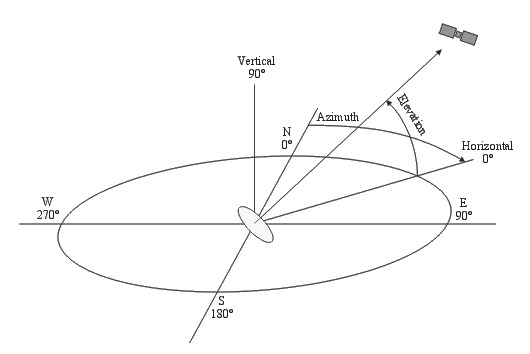
\includegraphics[Elevation and azimuth angle]{images/Elevation_and_azimuth_angle.jpg}
\newpage
\LARGE
Wave number\\
\normalsize
This defines the constant $k$ in terms of wavelength $\lambda$ as the wavelength is the distance on the
x-axis before the wave repeats itself. Thus, $k = 2\pi/\lambda$ is referred to as the
wave number.\cite{Fuller1995}\\\\
\LARGE
Transfer function\\
\normalsize
This refers to the rule by which an environment affects a signal.\cite{Regulinski1962}